\documentclass[12pt, titlepage]{article}

\usepackage{graphicx}
\usepackage{paralist}
\usepackage{amsfonts}
\usepackage{amsmath}
\usepackage{hhline}
\usepackage{booktabs}
\usepackage{multirow}
\usepackage{multicol}
\usepackage{booktabs}
\usepackage{tabularx}
\usepackage{hyperref}
\usepackage{float}
\usepackage{soul}


\hypersetup{
    colorlinks,
    citecolor=black,
    filecolor=black,
    linkcolor=red,
    urlcolor=blue
}
\usepackage[round]{natbib}

\title{SE 3XA3: Software Requirements Specification\\ChessAce}

\author{Team 18, Team MIF
		\\ Jerry Ke,  kex1
		\\ Harry Fu, fuh6
		\\ Morgan Cui, cuim2
}


\date{\today}

\begin{document}

\maketitle

\pagenumbering{roman}
\tableofcontents
\listoftables
\listoffigures

\begin{table}[bp]
\caption{\bf Revision History}
\begin{tabularx}{\textwidth}{p{3cm}p{2cm}X}
\toprule {\bf Date} & {\bf Version} & {\bf Notes}\\
\midrule
2018.10.05 & 0.1 & Draft\\
\color{red}{2018.11.23} & \color{red}{1.0} & \color{red}{Functional Requirement Revised}\\
\bottomrule
\end{tabularx}
\end{table}

\newpage

\pagenumbering{arabic}

\section{Project Drivers}

\subsection{The Purpose of the Project}
The purpose of this project is to re-implement the open source package ChessOOP. Large-scale video games are popular at present, but during the business days, most of the users, including students and employees, cannot enjoy such games with their insufficient fragmented time. Fortunately, people still have traditional board games like chess to utilize such spare time. Furthermore, chess can also help establish and enhance the relationship between different people. For example, two board game fans meet and choose to play chess during their study break. However, setting up the physical board and pieces usually depletes the limited time and the interest that appears occasionally. In this case, a portable, player versus player (PVP) chess program is needed to allow users to play it face to face anywhere anytime.

\subsection{The Stakeholders}

\subsubsection{The Client}
The client of the project is an external group who is acting as a evaluator and final viewer before its deployment. Such group of people may be interested in reverse-engineering or re-implement the project ChessAce in the later future.
\subsubsection{The Customers}
Consumers are individuals who will be interested in consuming the game content. The consumers, which members involve with all ages, who have the internet access to download the game, and the hardware support to interact with the game.
\subsubsection{Other Stakeholders}
Any other individuals, groups or organizations who have an interested in the game. Such entities mush have feasible tool to either interact with or investigate or modify the program following the software licensing.
\begin{itemize}
\item \textbf{Developer}: Members of MIF team are the developers for this project.
\end{itemize}


\subsection{Mandated Constraints}
\subsubsection{Solution Constraints}
\begin{itemize}
\item The program shall be implemented with Java language.
\item The program shall be able to download to and execute on any Windows, OS X and Linux OS with Java JDK.
\end{itemize}
\subsubsection{Implementation Environment of the Current System}
\begin{itemize}
\item The program shall be able to use any integrated PC display adapter to display graphic component.
\end{itemize}
\subsubsection{Partner or Collaborative Applications}
ChessAce does not have any direct partner or collaborative applications but does rely on Eclipse and some image editor to be implemented. It also relys on a personal computer supporting Java in order to execute.
\subsubsection{Off-the-Shelf Software}
For the product to execute, the following off-the-shelf software is required:
\begin{itemize}
\item Java
\end{itemize}
Java is free-to-download from online resource.
\subsubsection{Anticipated Workplace Environment}
The antocopated workplace environment is anywhere except extreme condition such as storm, rain or any other conditions that are capable of damaging the cooperating hardware.
\subsubsection{Schedule Constraints}
ChessAce must be completed with functional software and appropriate documentation in one university semester by December 8.
\subsubsection{Budget Constraints}
\textcolor{red}{The budget is not applicable to this project, since thet team will be using personal laptop to complete the code development. No addition resource is needed.}
\subsection{Naming Conventions and Terminology}
\begin{itemize}
\item Functional Requirements: Requirements that describes what the product will do
\item \textcolor{red}{Non-functional Requirements: Requirements that describe qualities that the product will have.}
\item ChessOOP: name of an open-source chess game program
\item \textcolor{red}{GUI: Graphical User Interface}
\item \textcolor{red}{shall: have to achieve}
\item \textcolor{red}{should: recommend to}

\end{itemize}

\subsection{Relevant Facts and Assumptions}

\subsubsection{Relevant Facts}
The application is intended for use by two users on their local machine. The length of the overall codes is approximately \textcolor{red}{2000} lines. The open-source project that the application is based upon has a very short revision history and part of documentation, and lacking a specific user manual.

\subsubsection{Business Rules}
The only rules \textcolor{red}{the team has} established is that everyone\textcolor{red}{shall} contribute approximately the same into the development, and members should take jobs if they feel they are stronger in certain areas.

\subsubsection{Assumption}
It will assume that the users will have general knowledge of computers. If the any advanced knowledge is needed, it  will be explained in a user manual. The developer has assumed that all the developing tool, such as IDE and image processing, etc, will be free. Also, the team has assumed that all the users are able to gain internet access in order to download the project.


X The open-source project that the application is based upon has a very short revision history and part of documentation, even lacking a specific user manual. This needs to be addressed in reimplementation. It will assume that the users only have basic general knowledge of computers. In order to use the application, any elements or features of the application whose operation requires more advanced knowledge will be explained in a user manual.

\section{Functional Requirements}

\subsection{The Scope of the Work and the Product}

\subsubsection{The Context of the Work}
\begin{figure}[H]
  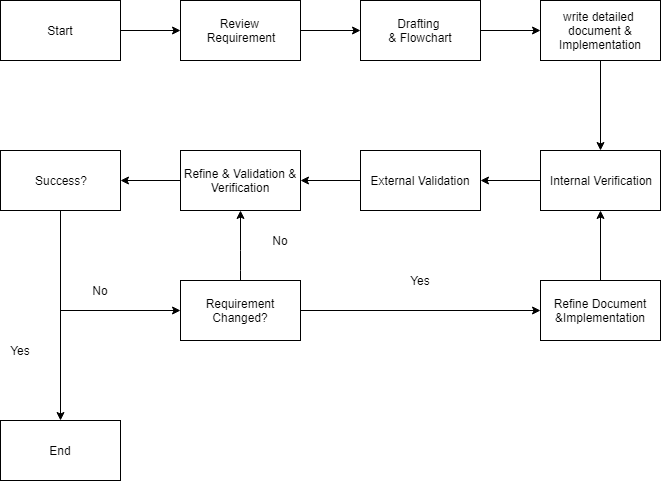
\includegraphics[width=\linewidth]{WorkContext.png}
  \caption{Flow chart for context of work.}
  \label{fig:context}
\end{figure}

\subsubsection{Work Partitioning}
\begin{table}[H]
\footnotesize
\begin{center}
\begin{tabular}{| l | l | l | l |}
\hline
\textbf{Event Number} & \textbf{Event Name} & \textbf{Input} & \textbf{Output}\\
\hline
1 & ChessAce Creation & Developer code & Java GUI Window\\
\hline
2 & ChessAce Movement Audio & Microphone, Audio file & Audio output device\\
\hline
3 & ChessAce Pieces Creation & Drawing Tool & Java GUI Window\\
\hline
4 & ChessAce Unit Elimination & Developer code & Java GUI Window\\
\hline
5 & ChessAce Checkmate\&Victory & Developer code and Image File &  Java GUI Window\\
\hline    
\end{tabular}
\normalsize
\caption{Work Partitioning 1}
   \label{tab:table}
\end{center}
\end{table}


\subsubsection{Individual Product Use Cases}
\begin{figure}[H]
  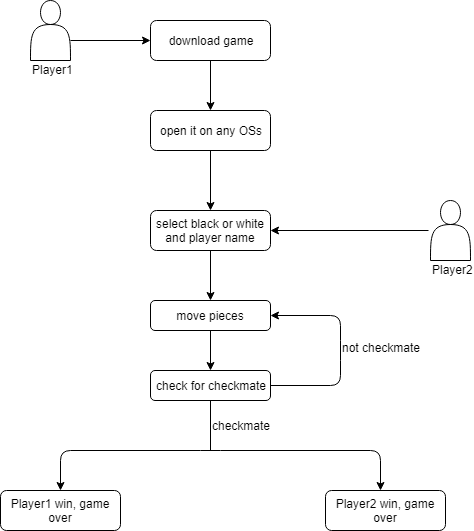
\includegraphics[width=\linewidth]{UseCase.png}
  \caption{Individual Product Use Case.}
  \label{fig:useCase}
\end{figure}
\subsection{Functional Requirements}
\begin{itemize}
\item \textbf{Requirement number}: FR1 \newline
 The user must be able to move pieces on chess board. \newline
Rationale: If the user cannot play this game on a standard chess board, then the program is not performing its basic function.
\item \textbf{Requirement number}: FR2   \newline
The system must show possible movement for chess pieces to user. \newline
Rationale: To allow the user to choose the possible movement for pieces. 
\item \textbf{Requirement number}: FR3  \newline
The system must perform unit elimination when user move one piece to the opponent’s piece.\newline
Rationale: To allow this game to perform the basic chess rules.
\item \textbf{Requirement number}: FR4 \newline
The user interface must show timer and current player. \newline
Rationale: To allow the user to manage their time and know whose term it is. 
\item \textbf{Requirement number}: FR5 \newline
This game must let two players to play at the same time. \newline
Rationale: The purpose of this game is this game is a player versus player offline chess game.
 
\item \textbf{Requirement number}: FR6 \newline
When one of the players have no movement can be done, the system show checkmate.\newline
Rationale: To allow this game end and show the result.
 
\item \textbf{Requirement number}: FR7\newline
The program must save the latest record of the game.\newline
Rationale: If the program cannot save the latest recording, then the program is not performing its required behaviour and is malfunctioning.
 
\item \textbf{Requirement number}: FR8\newline
The player who is playing white is the first one to move.\newline
Rationale: If not the player who playing white to move first, then the program does not comply with the chess rule.
 
\item \textbf{Requirement number}: FR9\newline
Users shall be able to download the executable jar and run it on any platform.\newline
Rationale: If this cannot be achieved, then the program is not performing its required behaviour.
 
\item \textbf{Requirement number}: FR10\newline
Users shall be able to start a game once two users are available. \newline
Rationale: To meet the goal of this project which is a PVP game.

\item \textbf{Requirement number}: FR11\newline
Users shall be given the choice of who plays black and white. \newline
Rationale: To improve the project’s performance.

\item \textbf{Requirement number}: FR12\newline
The inactive player may request to undo the prior move. \newline
Rationale: To allow this game to perform the basic chess rules.
 
\item \textbf{Requirement number}: FR13\newline
There shall be no more than one undo request per turn.\newline
Rationale: To meet the general chess rule.
 
\item \textbf{Requirement number}: FR14\newline
Captured pieces shall be displayed in a captured pieces box. \newline
Rationale: To improve the project’s readability.
 
\item \textbf{Requirement number}: FR15\newline
A player must be given a confirm dialog before forfeiting. \newline
Rationale: To avoid the user forfeiting the game by wrong click.
 
\item \textbf{Requirement number}: FR16\newline
The active player must receive information about the remaining time to make the next move.\newline
Rationale:  To remind the user left time and give a constraint to the program.
 
\item \textbf{Requirement number}: FR17\newline
The active player shall select a piece by clicking it. \newline
Rationale: To formulate the rules of the program.
 
\item \textbf{Requirement number}: FR18\newline
When a piece is selected, all legal moves for that piece are highlighted. \newline
Rationale: To improve the readability of the program.
 
\item \textbf{Requirement number}: FR19\newline
When a piece is selected, the active player may select another piece by clicking it. \newline
Rationale: To formulate the rules of the program.
\end{itemize}


\section{Non-functional Requirements}

\subsection{Look and Feel Requirements}
\begin{itemize}
\item The chess board of the product must look like the standard 8*8 chess board.
\item The game has to clearly label the pieces with white and black to distinguish sides.
\item The pieces shall have distinguish shapes to show their identities.
\end{itemize}

\subsection{Usability and Humanity Requirements}
\begin{itemize}
\item The set up menu shall be easy for anyone over 6 years old to use.
\item The game section shall be stratight forward for anyone who has a basic idea of chess play.
\item For players who never played chess before, an integrated rule manual shall be provided to assist.
\end{itemize}
\subsection{Performance Requirements}
\subsubsection{Speed Requirement}
\begin{itemize}
\item The initialization of the game shall not take more than 10 seconds.
\item All operation performed by player shall respond with a display change to indicate either a valid or an invalid operation under 0.5 seconds.
\end{itemize}
\subsubsection{Safety Critical Requirement}
\begin{itemize}
\item This execution process of this software is not related to any obvious physical hazards.
\end{itemize}
\subsubsection{Precision Requirement}
\begin{itemize}
\item The selected chess piece must move to the user selected valid square.
\item The player can only move the pieces of the pre-selected side.
\end{itemize}
\subsubsection{Reliability and Availability Requirement}
\begin{itemize}
\item The software must be able to initialize and operate normally, not necessarily continuously, at any time.
\end{itemize}
\subsection{Operational and Environmental Requirements}
\subsubsection{Expected physical environment}
\begin{itemize}
\item The software will be used by people, who will be sitting down, inside a climate controlled environement.
\end{itemize}
\subsubsection{Expected technical environment}
\begin{itemize}
\item Players will interface with the software through either a desktop or laptop, powered by windows, OS X, Linux or other operating system that has JAVA JDK.
\end{itemize}
\subsubsection{Partner Application}
\begin{itemize}
\item ChessAce must cooperate with the hardware integrated with the PC, such as CPU and RAM.
\end{itemize}
\subsection{Maintainability and Support Requirements}
\subsubsection{Maintainability}
\begin{itemize}
\item Each piece, chess board and restriction should all have their unique module.
\item Modules should keep the property of high cohesion low coupling.
\end{itemize}
\subsubsection{Portability}
\begin{itemize}
\item The program is expected to run on Linux, OS X, Windows and other operating systems with a Java JDK.
\end{itemize}
\subsection{Security Requirements}
\begin{itemize}
\item ChessAce shall not access unnecessary data on the user's device, and any accessed data, which is not generated by the program, shall not be able to upload, download to any cloud server or personal device.
\end{itemize}
\subsection{Cultural Requirements}
\begin{itemize}
\item ChessAce will not use any text, images, audio or other medias that will offend the ethnic group that purchase it.
\item ChessAce shall show a disclaimer explaining that any similarity to any cultural, ideology or political figure is coincidental.
\end{itemize}
\subsection{Legal Requirements}
\begin{itemize}
\item ChessAce shall comply with all national and federal software regulation laws.
\item ChessAce intelligent software shall comply with all relevant software standards.
\item ChessAce intelligent software shall comply with all relevant privacy acts.
\end{itemize}
\subsection{Health and Safety Requirements}
\begin{itemize}
\item After 2 hours of continuous usage, prompt message will suggest a rest with a frequency of 15 minutes.
\item After 3 hours of continuous usage, ChessAce will automatically terminate.
\end{itemize}

\section{Project Issues}

\subsection{Open Issues}
Automated Testing:
The ability to determine the correctness of the player's chess movement needs to be implemented to enable automated testing.
The ability to determine chess plate setting and checkmate (starting a game and ending game) needs to be implemented to enable automated testing.
\medskip \newline
Understanding code structure of existing open-source project:
The project that the application is based on has undocumented code with some unimplemented basic features, so analyzing its code structure is necessary to understand how the program functions.
\subsection{Off-the-Shelf Solutions}
There are many currently available product that are similar to the application. We could find many existing online or offline chess video game online, such as chess with friends, chess titans, Sparkchess. These chess game are all similar to our project which could help us to understand the basic rules of chess and to implement our player versus player offline chess game.

\subsection{New Problems}
N/A ATM

\subsection{Tasks}
The project's task is set by the deliverable outline for Software Engineering 3XA3. The final demonstration and documentation will need to complete by December 5th, 2018. Deliverables include ProjectApproval, DevelopmentPlan, ProblemStatement, Requirements Document Revision 0, Proof of Concept Demonstration, Test Plan Reversion 0, Design and Document Revision 0, Revision 0 Demonstration, Final Demonstration Revision 1, Peer Evaluation of Oher Team Final Demo and Final Documentation Revision 1.

\subsection{Migration to the New Product}
Requirements will be phased in over time in order of the priorities listed in this documentation, starting with High Priority requirements. The new product will be tested on three devices, running Windows 10, Linux, and Mac OS 10. The product should pass the current battery of automated unit testing as well.

\subsection{Risks}
One of the risks is that the project may crash because the player may do some misoperation such as move the chess pieces out of chess plate or did some movement which breaks the chess's role. These operations may cause the software crash which also means that the testing portion of the project will heavily rely on the user's operation and chess movements. The other risks may be a memory leak and make the whole system slowing down. This means the testing portion of the project will heavily rely on checking the memory state to make sure no stack overflow happens.

\subsection{Costs}
N/A ATM
\subsection{User Documentation and Training}
The product will contain a user manual which will include instructions on
how to use the application, the rules of chess movement and it will include details on all of its features
and options.
\subsection{Waiting Room}
The GUI needs to be improved and the functional and non-functional re-
quirements need to be implemented.
\subsection{Ideas for Solutions}
Using GUI development software could help improve the GUI.



\bibliographystyle{plainnat}

\bibliography{SRS}

\newpage

\section{Appendix}

N/A ATM

\subsection{Symbolic Parameters}

N/A ATM


\end{document}
